\documentclass[dvisvgm,hypertex,aspectratio=169]{beamer}
\usefonttheme{serif}

%\usepackage[draft]{animate}
\usepackage[final]{animate}
\usepackage{ifthen}


%%%%%%%%%%%%%%%%%%%%%%%%%%%%%%%%%%%%%%%%%%%%%%%%%%%%%%%%%%%%%%%%%%%%%%%%%%%%%%%
% PageDown, PageUp key event handling; navigation symbols
%%%%%%%%%%%%%%%%%%%%%%%%%%%%%%%%%%%%%%%%%%%%%%%%%%%%%%%%%%%%%%%%%%%%%%%%%%%%%%%
\usepackage[totpages]{zref}
\usepackage{atbegshi}
\usepackage{cancel}
\usepackage{fontawesome}
\setbeamertemplate{navigation symbols}{}
\AtBeginShipout{%
  \AtBeginShipoutAddToBox{%
    \special{dvisvgm:raw
      <defs>
      <script type="text/javascript">
      <![CDATA[
        document.addEventListener('keydown', function(e){
          if(e.key=='PageDown'){
            \ifnum\thepage<\ztotpages
              document.location.replace('\jobname-\the\numexpr\thepage+1\relax.svg');%
            \fi
          }else if(e.key=='PageUp'){
            \ifnum\thepage>1
            %document.location.replace('\jobname-\the\numexpr\thepage-1\relax.svg');%
              document.location.replace('\jobname-\makeatletter\@anim@pad{2}{\thepage-1}\makeatother\relax.svg');%
            \fi%
          }
        });
      ]]>
      </script>
      </defs>
    }%
  }%
  \AtBeginShipoutUpperLeftForeground{%
    \raisebox{-\dimexpr\height+0.5ex\relax}[0pt][0pt]{\makebox[\paperwidth][r]{%
      \normalsize\color{structure!40!}%
      \ifnum\thepage>1%
      \href{\jobname-\the\numexpr\thepage-1\relax.svg}{\faArrowLeft}%
      \else%  
        \textcolor{lightgray}{\faArrowLeft}%  
      \fi\hspace{0.5ex}%
      \ifnum\thepage<\ztotpages%
      \href{\jobname-\the\numexpr\thepage+1\relax.svg}{\faArrowRight}%
      \else%
        \textcolor{lightgray}{\faArrowRight}%  
      \fi%
      \hspace{0.5ex}%
    }}%
  }%  
}%
%%%%%%%%%%%%%%%%%%%%%%%%%%%%%%%%%%%%%%%%%%%%%%%%%%%%%%%%%%%%%%%%%%%%%%%%%%%%%%%

\usepackage{tikz}
\usepackage{pgfplots}
\usepackage{pgfplotstable}
\pgfplotsset{compat=1.16}
\usetikzlibrary{calc}
\usepackage{amsmath}
\DeclareMathOperator{\sign}{sgn}


\author{Kjartan Halvorsen}
\date{2022-05-16}
\title{Modeling and automation}

% ------------------------------------------------
% Determine which slides to include
\includeonlyframes{%
  Ex0,% Control
  I00,% Control
%I01,% Control
  A0,% Sistemas mecánicos
  A1,% Modelación es encontrar descripción matematica
  A1E,% Hummer animation. Free-body diagram
  A1S,% Hummer animation. Free-body diagram solution
  I1E,% Intuición
  I1S,% Intuición, solución
  M1,% Como modelar?
  M2,% Simplificar
  M3,% Modelo de masa puntal
  M30,% Modelo de masa puntal
  M4,% Modelo de arrastre
  M5E,% Respuesto de escalón
  M6A,% Respuesta, animación
  L1,% Linearización
  L2A,% Linearización local
  Ex1,% Linearización local
%L2E,% Linearización cuatro alternativas. Cuál es mejor
%M8,% Solución del sistema lineal
%M9,% Transforme de Laplace
%M10,% Polo y respuesta
}
% ------------------------------------------------

%%%%%%%%%%%%%%%%%%%%%%%%%%%%%%%%%%%%%%%%%%%%%%%%%%%%%%%%%%%%%%%%%%%%%%%%%%%%%%%
% Define footer
\usepackage{ccicons}

\makeatletter
\setbeamertemplate{footline}
{
  \leavevmode%
  \hbox{%
  %\begin{beamercolorbox}[wd=.333333\paperwidth,ht=2.25ex,dp=1ex,center]{title in head/foot}%
    %\usebeamerfont{title in head/foot}\insertsubsection
  %\end{beamercolorbox}%
  %\begin{beamercolorbox}[wd=.333333\paperwidth,ht=2.25ex,dp=1ex,right]{date in head/foot}%
  %  \usebeamerfont{date in head/foot}\insertshortdate{}\hspace*{2em}
  %  \insertframenumber{} / \inserttotalframenumber\hspace*{2ex} 
  %\end{beamercolorbox}}%
  %\vskip0pt%
  \begin{beamercolorbox}[wd=.92\paperwidth,ht=2.25ex,dp=1ex,right]{author in head/foot}%
    \usebeamerfont{author in head/foot}\insertauthor
  \end{beamercolorbox}%
  \begin{beamercolorbox}[wd=.08\paperwidth,ht=2.25ex,dp=1ex,right]{date in head/foot}%
    \ccbysa
  \end{beamercolorbox}}%
  \vskip0pt%
}
\makeatother
%%%%%%%%%%%%%%%%%%%%%%%%%%%%%%%%%%%%%%%%%%%%%%%%%%%%%%%%%%%%%%%%%%%%%%%%%%%%%%%


\newcommand{\hummeranimation}[1]{%

  \def\velocity{1.5}
  \def\startbrake{3}
  \def\braketimeconst{3}

  \begin{center}

  %\begin{animateinline}[controls,autoplay,loop]{20}
  \begin{animateinline}[ ]{28}
      \multiframe{60}{n=0+0.15}{
        \begin{tikzpicture}
          \useasboundingbox (-1 cm, -1 cm) rectangle (9 cm, 3 cm);
          \pgfmathsetmacro{\xpos}{\velocity*\n*(\n<\startbrake) + (\velocity*\startbrake + \velocity*\braketimeconst*(1-(exp(-(\n-\startbrake)/\braketimeconst))))*(\n >= \startbrake)}

            \node[anchor=south,] at (\xpos cm, 0) {\ifnum#1 > 0 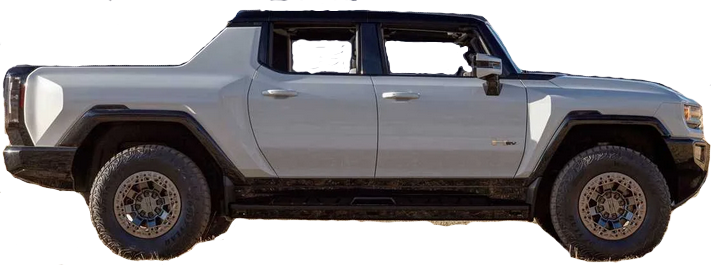
\includegraphics[width=15 mm]{hummer-ev.png} \else \tikz \draw[fill, black] (0,0) rectangle (1,1); \fi};
            \draw[->, black!90, semithick] (-1, 0.16) -- (9 , 0.16) node[below, pos=1] {$X$};
        \end{tikzpicture}
      }
    \end{animateinline}
  \end{center}
}

\begin{document}

\maketitle

\begin{frame}[label=Ex0]{A mechatronic system}

  \begin{center}
    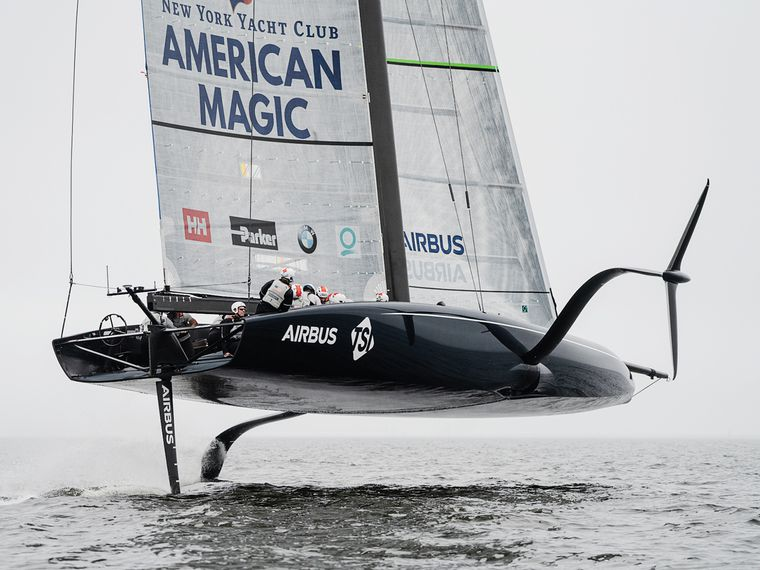
\includegraphics[height=0.7\textheight]{ac75.jpeg}\\
    {\footnotesize  From SailingWorld}
  \end{center}

  AC75 Class
\end{frame}

\begin{frame}[label=I00]{Control systems}

\begin{center}
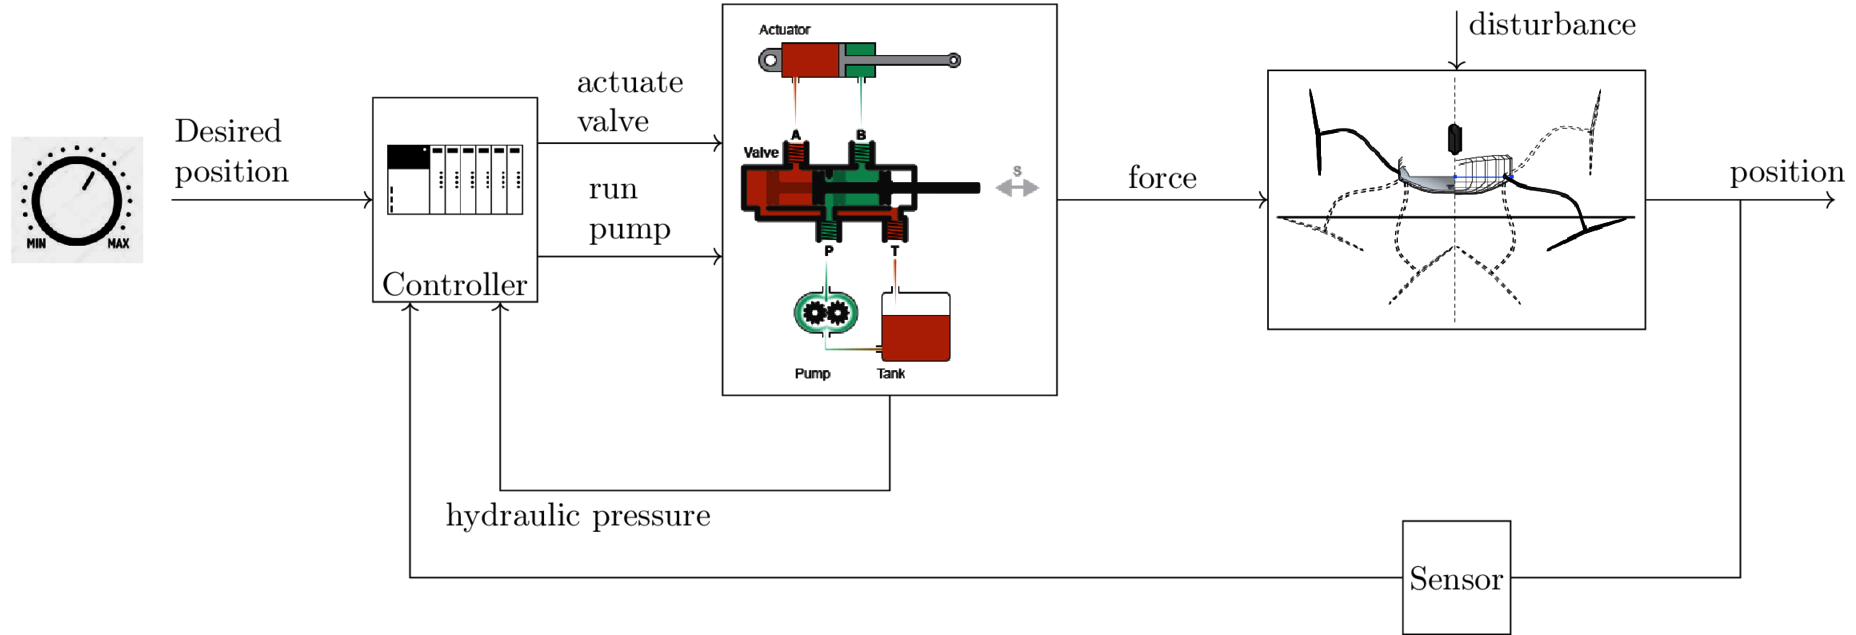
\includegraphics[width=1.0\textwidth]{ac75-control-block-details.png}
\end{center}

  % \begin{center}
  %   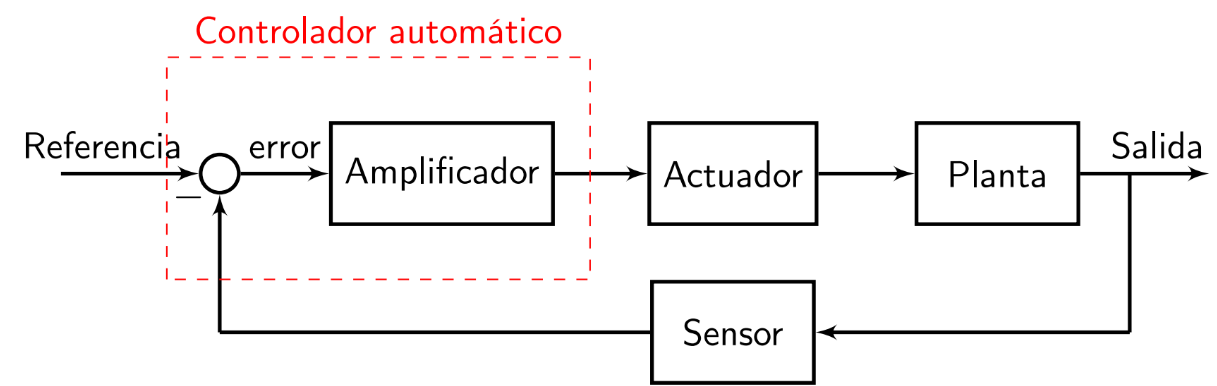
\includegraphics[width=0.7\linewidth]{minchala-block-control.png}\\
  %   {\tiny Source: Prof Ismael Minchala, Tec}
  % \end{center}
\end{frame}


\note{%
}

\begin{frame}[label=I01]{Why control?}
  \begin{center}
    
\includegraphics[width=8cm]{pirelli.jpg}
  \end{center}
  
\end{frame}



\begin{frame}[label=A1]{A mechanical system}

  
  \hummeranimation{1}

  \alert{Activity} Identify and indicate with arrows all the forces that act on the car. For each force identify and indicate its counter-force (according to Newton's third law). 

\end{frame}


\note{%
}

\begin{frame}[label=I1E]{Intuition about mechanical systems}

  A car is traveling on a horizontal road at constant velocity. At the instant $t=t_1$, the driver shifts the transmission to neutral ('N'), thereby disconnecting the motor from the wheels. Which of the following graphs best describe the behavior of the car's \textbf{velocity} $v(t)=\frac{d}{dt}X(t)$?

  \pause
  
  \begin{center}
    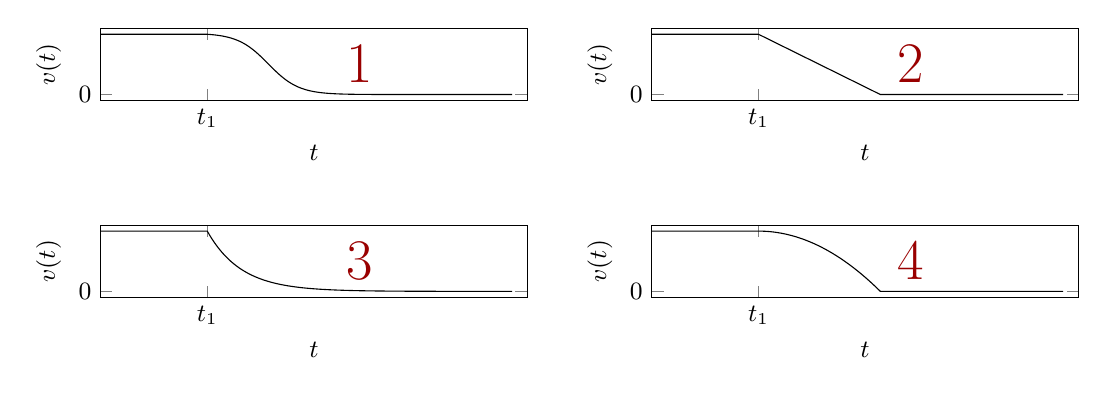
\begin{tikzpicture}
      \small

      \begin{axis}[
        width=7cm,
        height=2.5cm,
        xlabel={$t$},
        ylabel={$v(t)$},
        xmin=-3.5,
        xmax=10.5,
        ytick = {0},
        xtick = {0},
        xticklabels = {$t_1$},
        ]
        \addplot+[black, no marks, domain=-4:10, samples=400,variable=k] { (k < 0) + (k>0)*(1+exp(-4))/(1+exp(4*(0.5*k-1)))};

        \node[black!40!red] at (axis cs: 5, 0.5) {\huge 1};
      \end{axis}

      \begin{axis}[
        xshift=7cm,
        width=7cm,
        height=2.5cm,
        xlabel={$t$},
        ylabel={$v(t)$},
        xmin=-3.5,
        xmax=10.5,
        ytick = {0},
        xtick = {0},
        xticklabels = {$t_1$},
        ]
        \addplot+[black, no marks, domain=-4:10, samples=400,variable=k] { (k<0) + ((k>=0) - (k>4))*(1/4*(4-k)) };
        \node[black!40!red] at (axis cs: 5, 0.5) {\huge 2};
      \end{axis}

      \begin{axis}[
        xshift=0cm,
        yshift=-2.5cm,
        width=7cm,
        height=2.5cm,
        xlabel={$t$},
        ylabel={$v(t)$},
        xmin=-3.5,
        xmax=10.5,
        ytick = {0},
        xtick = {0},
        xticklabels = {$t_1$},
        ]
        \addplot+[black, no marks, domain=-4:10, samples=400,variable=k] { (k<0) + (k>0)*exp(-0.9*k)};
        \node[black!40!red] at (axis cs: 5, 0.5) {\huge 3};
      \end{axis}

      \begin{axis}[
        xshift=7cm,
        yshift=-2.5cm,
        width=7cm,
        height=2.5cm,
        xlabel={$t$},
        ylabel={$v(t)$},
        xmin=-3.5,
        xmax=10.5,
        ytick = {0},
        xtick = {0},
        xticklabels = {$t_1$},
        ]
        \addplot+[black, no marks, domain=-4:10, samples=400,variable=k] { (k<0) + ((k>=0) - (k>4))*(1-1/16*pow(-k,2)) };
        \node[black!40!red] at (axis cs: 5, 0.5) {\huge 4};
      \end{axis}


    \end{tikzpicture}

  \end{center}

\end{frame}

\begin{frame}[label=M1]{Modeling}

  \hummeranimation{1}

  \begin{center}
    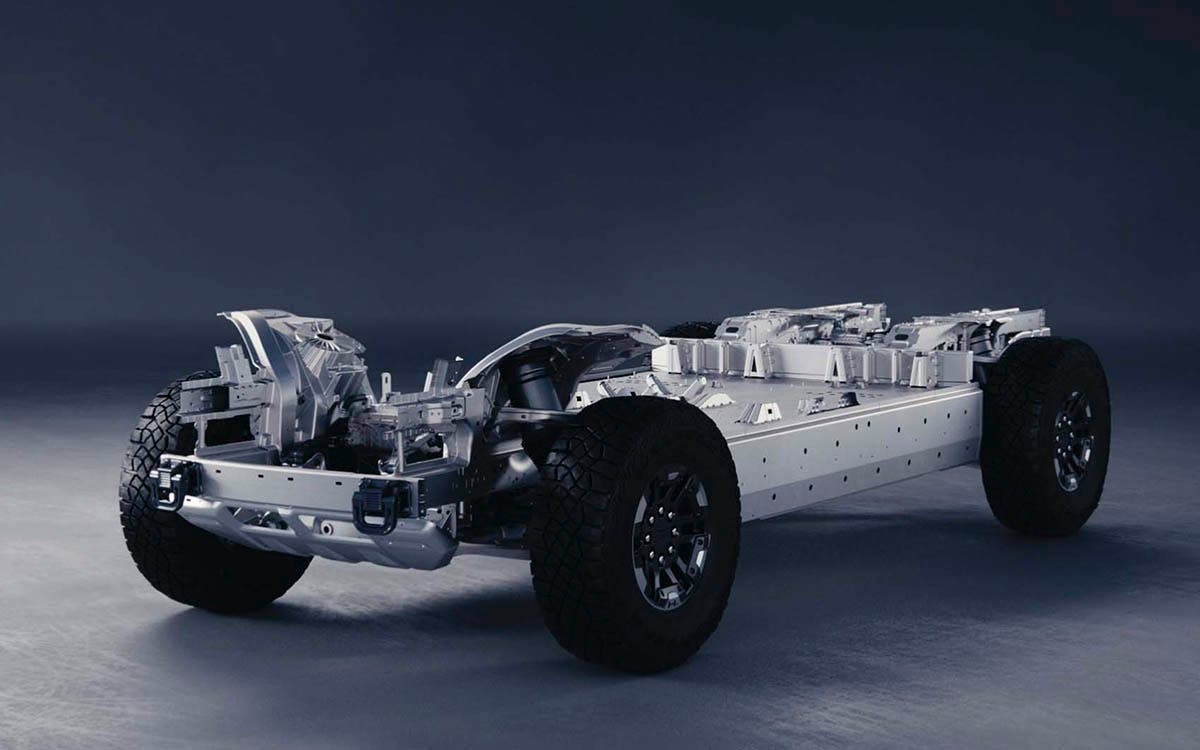
\includegraphics[height=2cm]{hummer-ev.jpg}
  \end{center}
  How should we \alert{model} this system?

  \pause
  
  It depends. But on what?

  \pause

  On the \alert{purpose}: What do want the model for?
\end{frame}

\note{%
  Para este ejemplo el contexto de la modelación, o el propósito es el diseño de un controlador para mantener la velocidad. Un cruise control.
}

\begin{frame}[label=M2]{Simplification}

  \hummeranimation{0} % Just black box

\end{frame}

\note{%
  Evidentemente este es una simplificación enorme de lo que es un Hummer EV. Pero va a ser suficiente para llegar a un modelo adecuado para diseñar un controlador de velocidad.
}

\begin{frame}[label=M3]{Point-mass model}

  \footnotesize 
  
  Newton's second law: ``The rate of change of the momentum is equal to the sum of forces''
  \[ \frac{d}{dt} (mv) = \sum_i F_i\]
  \begin{center}
    \footnotesize
    %\begin{tikzpicture}[scale=1.2, transform shape]
    \begin{tikzpicture}[scale=.8]
      \node[anchor=south,] at (1, 0) (hummer) {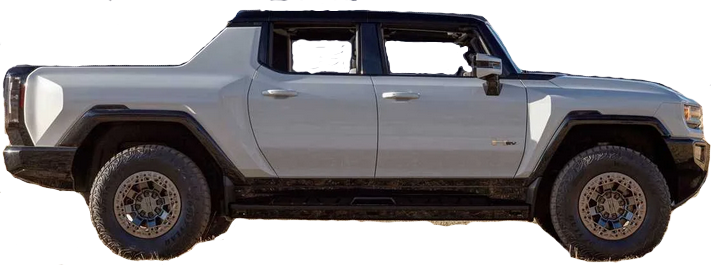
\includegraphics[width=15 mm]{hummer-ev.png}};
      \node[coordinate] (com) at ($ (hummer.center) + (0.15, 0) $) {};
      \node[coordinate] (wheels) at ($ (hummer.south) + (0, 0.16) $) {};
      
      \draw[->, black!90, semithick] (-1, 0.16) -- (9 , 0.16) node[below, pos=1] {$X$};
      \draw[->, black!90, ] (-1, 0.16) -- (-1 , 3) node[left, pos=1] {$Y$};
      
      \draw[thick, green!70!black, ->] (com) -- ++(0, -2cm) node[right] {$F_g = mg$};
      \draw[thick, orange!80!black, ->] (wheels) -- ++(0, 2cm) node[right] {$F_{n}$};
      \draw[thick, red!80!black, ->] (wheels) -- ++(2cm, 0) node[below] {$F_m$};
      \draw[thick, blue!80!black, <-] (hummer.east) -- ++(2cm, 0) node[above] {$F_d$};

    \end{tikzpicture}
  \end{center}

  \pause
  
  No acceleration in the $Y$-direction (forces in equilibrium)
  \[ 0 = F_{n} - F_g \quad \Rightarrow \quad F_{n} = F_g = mg\]
  \pause
  In the $X$-direction:
  \[ m\dot{v} = F_m - F_d\]
\end{frame}

\note{%
  En verdad la simplificación es más de lo que está visualizado con una caja. No nos importa en este modelo la distribución de fuerzas en el superficie de la caja. Entonces estamos asumiendo de que toda la masa está concentrado en un punto, y de que todas las fuerzas actuan en este punto. 
}

\begin{frame}[label=M30]{... and climbing from Cuernavaca towards Tres Marías...}

  \begin{center}
    \footnotesize
    \begin{tikzpicture}[scale=1.2, transform shape]

      \begin{scope}[rotate=10,]
      \node[anchor=south,] at (1, 0) (hummer) {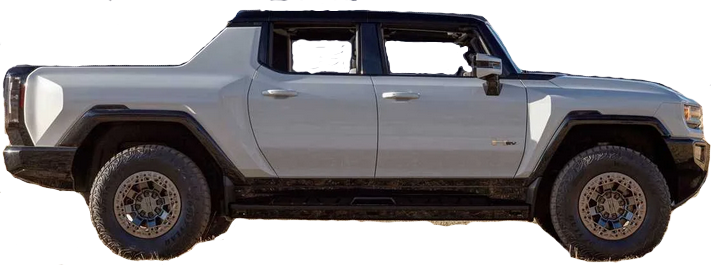
\includegraphics[width=15 mm]{hummer-ev.png}};
      \node[coordinate] (com) at ($ (hummer.center) + (0.15, 0) $) {};
      \node[coordinate] (wheels) at ($ (hummer.south) + (0, 0.16) $) {};
      
      \draw[->, black!90, semithick] (-1, 0.16) -- (9 , 0.16) node[below, pos=1] {$X$};
      \draw[->, black!90, ] (-1, 0.16) -- (-1 , 3) node[left, pos=1] {$Y$};
      
      \draw[thick, green!70!black, ->, rotate=-10] (com) -- ++(0, -2cm) node[right] {$F_g = mg$};
      \draw[thick, orange!80!black, ->] (wheels) -- ++(0, 2cm) node[right] {$F_{n}$};
      \draw[thick, red!80!black, ->] (wheels) -- ++(2cm, 0) node[below] {$F_m$};
      \draw[thick, blue!80!black, <-] (hummer.east) -- ++(2cm, 0) node[above] {$F_d$};
    \end{scope}
    \draw[dashed] (-1,0) to (9, 0);
    \draw[->] (4, 0) arc[radius=5cm, start angle=0, end angle=10] node[right, pos=0.5] {$\theta$};
  \end{tikzpicture}
  \end{center}

\end{frame}

\note{%
  Nota de que cuando está inclinado el suelo, lo único que cambia es que ahora la fuerza de gravidad tiene un componente en la dirección de la velocidad del coche. El sistema de referencia mejor para analyzar la situación todavía tiene un eje en la dirección del coche, y el otro perpendicular.
}


\begin{frame}[label=M4]{Friction model}
  \begin{columns}
    \begin{column}{0.5\linewidth}
      \[ m\dot{v} = F_m - F_d\]
      Quadratic friction model \(F_d = \sign(v)kv^2\).

      \[ m\dot{v} + \sign(v)kv^2 = F_m\]
      \alert{Nonlinear differential equation.}
    \end{column}
    \begin{column}{0.5\linewidth}
    \begin{center}
    \begin{tikzpicture}
      \begin{axis}[
        axis lines = middle,
        ytick=\empty,
        xtick=\empty,
        xlabel={$v$},
        ylabel={$F_d$},
        ]
        
        \addplot [blue!80, smooth, domain=-4:4] { sign(x)*x*x};

      \end{axis}
    \end{tikzpicture}
  \end{center}
\end{column}
\end{columns}
\end{frame}

\note{%
  Vamos a enfocarnos en la fuerza de arrastre. A partir de cierta velocidad, el arrastre del viento es la mayor resistencia al movimiento del coche. Esta resistencia crece con la cuadrada de la velocidad relativa entre el coche y el aire. Es decir que si la duplicamos la velocidad, la resistencia será cuatro veces más grande.
  De que depende el coeficiente k? (densidad del aire, forma del coche, area frontal => drag coefficient).
}

 \pgfplotstableread[col sep=comma]{car-drag-60.dta}{\cardragtable}

\begin{frame}[label=M5E]{Point-mass model}

  \[ m\dot{v} = F_m - \sign(v)kv^2\]

  Initially, the car is stationary. At time instant $t=0$ the force generated by the motor rises immediately from $F_m=0$ to $F_m=F_0$  and kept constant. How does the system respond?

    \begin{center}
    \begin{tikzpicture}
      \small

      \begin{axis}[
        width=7cm,
        height=2.5cm,
        xlabel={$t$},
        ylabel={$v(t)$},
        xmin=-0.5,
        xmax=6,
        ytick = {0},
        xtick = {0},
        %xticklabels = {$t_1$},
        ]
        \addplot+[black, no marks, domain=-1:6, samples=200, smooth, variable=k] { (k>=0)*(exp(1.6*(k-3))/(1+exp(1.6*(k-3))))};

        \node[black!40!red] at (axis cs: 5, 0.5) {\huge 1};
      \end{axis}

      \begin{axis}[
        xshift=7cm,
        width=7cm,
        height=2.5cm,
        xlabel={$t$},
        ylabel={$v(t)$},
        xmin=-0.5,
        xmax=6,
        ytick = {0},
        xtick = {0},
        %xticklabels = {$t_1$},
        ]
        \addplot+[black, no marks, smooth] table[col sep=comma, y index = 2] {car-drag.dta};
        \node[black!40!red] at (axis cs: 5, 1) {\huge 2};
      \end{axis}

      \begin{axis}[
        xshift=0cm,
        yshift=-2.5cm,
        width=7cm,
        height=2.5cm,
        xlabel={$t$},
        ylabel={$v(t)$},
        xmin=-0.5,
        xmax=6,
        ytick = {0},
        xtick = {0},
        %xticklabels = {0},
        ]
        \addplot+[black, no marks, domain=-4:10, samples=100, smooth, variable=k] { (k>0)*(k<4)*(1/4*k) + (k>4) };
        \node[black!40!red] at (axis cs: 5, 0.5) {\huge 3};
      \end{axis}

      \begin{axis}[
        xshift=7cm,
        yshift=-2.5cm,
        width=7cm,
        height=2.5cm,
        xlabel={$t$},
        ylabel={$v(t)$},
        xmin=-0.5,
        xmax=6,
        ytick = {0},
        xtick = {0},
        %xticklabels = {$t_1$},
        ]
        \addplot+[black, no marks, domain=-4:10, samples=100, smooth, variable=k] { (k>0)*(k<4)*1/16*pow(k,2)) + (k>4) };
        \node[black!40!red] at (axis cs: 5, 0.5) {\huge 4};
      \end{axis}
    \end{tikzpicture}
  \end{center}
\end{frame}

\begin{frame}[label=M6A]{Point-mass model}
  \[ \dot{v} = \frac{1}{m}(F_0 - \sign(v)kv^2) \]
  \begin{center}
    \begin{animateinline}[]{20}
      \multiframe{60}{n=1+1}{
        \pgfplotstablegetelem{\n}{2}\of\cardragtable
        \pgfmathsetmacro{\xpos}{\pgfplotsretval}
        \begin{tikzpicture}
          \begin{axis}[%
            axis lines = middle,
            ytick={4},
            yticklabels={$\frac{F_0}{m}$},
            xtick=\empty,
            xlabel={$v$},
            ylabel={$\dot{v}$},
            ymax=5,
            clip=false,
            ]
            \addplot [orange!80, smooth, domain=0:2.4] {4-sign(x)*x*x};
            \draw[blue!70, fill] (axis cs: \xpos, 0) circle[radius=5pt];
          \end{axis}
        \end{tikzpicture}
      }
    \end{animateinline}
  \end{center}
\end{frame}

\note{%
  El modelo es en forma de una ecuación diferencial non-lineal. En general se puede decir que el conjunto de EDs nonlineales que tiene una solución explicita (es decir en forma de funciones) es minusculo. La gran gran mayoría de ED nonlinales no tienen solución explicita. Pero esto no es decir que no podemos analizar y entender la ecuación. Un herramiento es este tipo de diagrama.

  Aquí veen un eje v, que representa la velocidad del coche, y un eje que representa la derivada de la velocidad, es decir, la acceleración. La ED nos dice que la acceleración depende de la velocidad según esta funcion, que es, nonlineal. La función está graficada. Entonces para cada valor de velocidad, podemos evaluar la function de la acceleración, que es este valor. Y este valor, sea positiva o negativo, y con cierta magnitud, nos dice como cambiará la velocidad, si el coche se encuentra con esta velocidad.

  Se puede visualisar con flechas en el eje v.

  Entonces vemos claramente que hay una velocidad de equilibrio, cuando la fuerza del motor y la resistencia del viento estan iguales.

  Tambien vemos que este equilibrio es estable.

  Entonces este herramiento nos da mucha información relevante sobre el comportamiento del sistema. Sin calcular la solución explicita.

  Pero siempre se puede resolver la DE de manera númerica, aunque no tiene solución explicita.
}

\begin{frame}[label=L1]{Linearization of the friction model}

  \[ m\dot{v} = F_m - F_d\]
  Friction model including rolling resistance \(F_d = \sign(v)(r + kv^2)\).
  \[ m\dot{v} = F_m -\sign(v)(r + kv^2)\]
  
\begin{center}
    \begin{tikzpicture}[scale=0.7]
      \begin{axis}[
        axis lines = middle,
        ytick=\empty,
        xtick=\empty,
        xlabel={$v$},
        ylabel={$F_d$},
        ]
        \addplot [blue!80, domain=-4:4, samples=800] { sign(x)*(0.4 + x*x)};
      \end{axis}
    \end{tikzpicture}
  \end{center}
  Problem: The design and analysis of the closed-loop system requires a \alert{linear model}. The model above is \alert{nonlinear}.

\end{frame}


\begin{frame}[label=L2A]{Linearization}
  \footnotesize
  \begin{columns}
    \begin{column}{0.6\columnwidth}
      \[ m \dot{v} = F_m - F_d = \underbrace{F_m - \sign(v)(r + kv^2)}_{f(v, F_m)} = f(v, F_m)\]
      \begin{enumerate}
         \item Define deviation variables.
        \[ F_m(t) = F_{m_0} + u(t), \quad v(t) = v_0 + y(t)\]
        \pause
      \item Choose operating point corresponding to equilibrium \(f(v_0, F_{m_0}) = 0\).
        \[ F_{m_0} -  \sign(v_0)(r + kv_0^2) = 0\]
        \pause
      \item  Do Taylor expansion of \(f(v, F_m)\).
        \begin{align*}
        f(v, F_m) &\approx \cancelto{0}{f(v_0, F_{m_0})} + \frac{\partial f}{\partial v}\big|_{v_0, F_{m_0}} \underbrace{(v - v_0)}_{y} + \frac{\partial f}{\partial F_m}\big|_{v_0, F_{m_0}} \underbrace{(F_m - F_{m_0})}_{u} 
      \end{align*}
      \pause
      \begin{align*}
        \frac{\partial f}{\partial v} &= -\begin{cases} 2kv, & v>0\\-2kv, & v<0\\\text{undefined}, & v=0 \end{cases}
      \end{align*}
    \end{enumerate}
  \end{column}
  \begin{column}{0.4\columnwidth}
    \pause
    \begin{enumerate}
      \setcounter{enumi}{3}
    \item Obtain linear ODE
      \begin{align*}
        m\frac{d}{dt} v &= m\frac{d}{dt} (v_0 + y) = m\frac{d}{dt} y = F_m - F_d
                          \approx u - 2kv_0y\\
        m\dot{y} &= -2kv_0y + u
      \end{align*}
    \end{enumerate}

    \pause
    
  %   \begin{center}
  %   \begin{animateinline}[controls, palindrome]{2}
  %     \multiframe{15}{n=-2.8+0.44}{
  %       \begin{tikzpicture}[scale=0.8]
  %       \pgfmathsetmacro{\vnull}{\n}
  %       \pgfmathsetmacro{\Fnull}{sign(\vnull)*(0.4+\vnull*\vnull)}
  %         \begin{axis}[
  %           axis lines = middle,
  %           ytick={\Fnull},
  %           yticklabels={$F_d(v_0)$},
  %           xtick={\vnull},
  %           xticklabels={$v_0$},
  %           xlabel={$v$},
  %           ylabel={$F_d$},
  %           clip=false,
  %           xmin=-6,
  %           xmax=6,
  %           ymin=-20,
  %           ymax=20,
  %           ]
           
  %           \addplot [blue!80, domain=-4:4, samples=400, thick] { sign(x)*(0.4 + x*x)};
  %           %\addplot [orange!80, domain=-1.5:1.5, samples=4, variable=\t] ({t}, {t});
  %           \addplot [orange!80, domain=-1.5:1.5, samples=4, variable=\t, thick] ({t+\vnull}, {sign(\vnull)*(0.4 + pow(\vnull, 2)) + (2*abs(\vnull))*t} );
  %         \end{axis}
  %       \end{tikzpicture}
  %     }
  %   \end{animateinline}
  % \end{center}
 \end{column} 
\end{columns}
\end{frame}

\note{%
  Ya llegamos al concepto más importante de esta sesión primera: Como llegar de un modelo non-lineal a un modelo lineal.

  1) Un modelo lineal sería una linea recta. Depende de que es la velocidad del coche hay un gran variedad de lineas rectas que aproximan bien la relación non-lineal.
  
  2) Entonces, tenemos que definir cuál es nuestro punto de operación v0. Suponemos que es una velocidad positiva.

  3) Definimos el variable de desviación. v = v0 + y   <=> y = v-v0

  4) Hacemos el series de Taylor alrededor del punto de operación v0, solo el termino constante y el termino linel.

  5) Substituimos la aproximación lineal en la ED original. 
}

\begin{frame}[label=Ex1]{Linearization exercise: Level-control of a tank}

  \footnotesize
  
  \begin{center}
    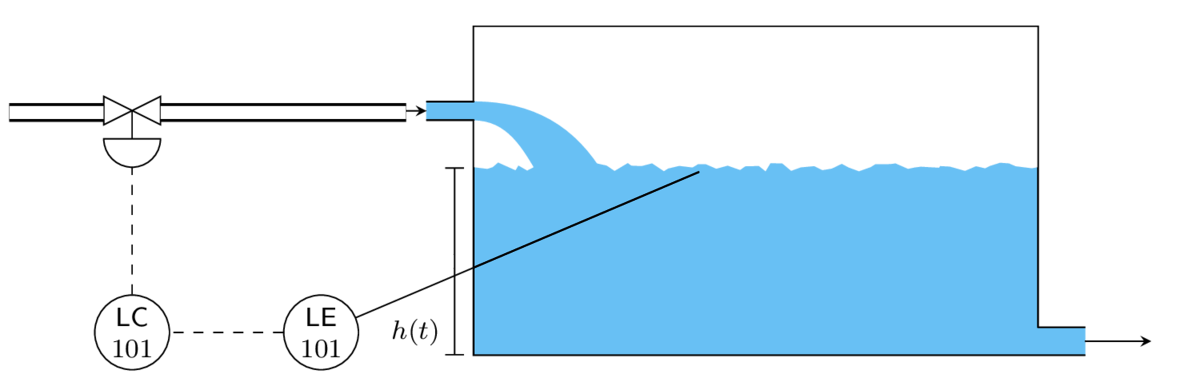
\includegraphics[width=0.5\linewidth]{tank-with-valve.png}
  \end{center}

  \begin{columns}
    \begin{column}{0.6\columnwidth}

      \begin{align*}
        \frac{d}{dt} V &= \text{flow in} - \text{flow out}\\
        \frac{d}{dt} Ah(t) &= Q_{in}(t) - Q_{out}(t)\\
        &= \gamma a(t) \sqrt{\Delta P(t)} - Q_{out}(t) = f(a, \Delta P, Q_{out})
      \end{align*}
    \begin{enumerate}
      \item Define deviation variables.
        \begin{align*} a(t) &= a_0 + u(t), \quad h(t) = h_0 + y(t),\\
          \quad \Delta P(t) &= \Delta P_0 + v(t),
                              \quad Q_{out}(t) = Q_0 + w(t)
        \end{align*}
      \end{enumerate}

    \end{column}

    \begin{column}{0.5\columnwidth}

      \begin{enumerate}
      \setcounter{enumi}{1}
      \item Choose operating point corresponding to equilibrium \(f(a_0, \Delta P_0, Q_0) = 0\).
        \[ \gamma a_0 \sqrt{\Delta P_0} - Q_0 = 0\]
    \item  Do Taylor expansion of \(f(a, \Delta P, Q_{out})\).
%      \begin{align*}
%        f(v, F_m) &\approx \cancelto{0}{f(v_0, F_{m_0})} + \frac{\partial f}{\partial v}\big__{v_0, F_{m_0}} \underbrace{(v - v_0)}_{y} + \frac{\partial f}{\partial F_m}\big__{v_0, F_{m_0}} \underbrace{(F_m - F_{m_0})}_{u} 
%      \end{align*}

%      \begin{align*}
%        \frac{\partial f}{\partial v} &= -\begin{cases} 2kv, & v>0\\2kv, & v<0\\\text{undefined}, & v=0 \end{cases}
%      \end{align*}
%      \pause
      \item Obtain linear ODE
%      \begin{align*}
%        m\frac{d}{dt} v &= m\frac{d}{dt} (v_0 + y) = m\frac{d}{dt} y = F_m - F_d
%                          \approx u - 2kv_0y\\
%        m\dot{y} &= -2kv_0y + u
%      \end{align*}
    \end{enumerate}
  

      
    \end{column}
  \end{columns}

\end{frame}


\end{document}
